\chapter{Introduction and Motivation}
\thispagestyle{plain}

\label{Introduction and Motivation}

% general aims. What are we trying to accomplish? We are trying to provide researchers and users of ABMs insight into the workings of ABMs.
% Definition of ABM.
% Developed a framework that learns both a forward mapping and a reverse mapping of a system.
% These mappings can be used to predict and control behavior in a ABM.
The behavior of individual agents in an agent-based model (ABM) is typically well understood because the agent's program directly controls its local behaviors.
What is typically not understood is how changing these programs' agent-level control parameters affect the observed system-level behaviors of the ABM.
The aim of this dissertation is to provide researchers and users of ABMs insight into how these agent-level parameters affect system-level properties.
I present a learning framework, the \framework (\fw), that can be used to predict and control system-level behaviors of agent-based models.
Using this framework, users can interact with ABMs in terms of intuitive system-level concepts, instead of with agent-level controls that only indirectly affect system-level behaviors.


\section{Agent-Based Models}

% ABMs, according to their definition are governed by the agent-based programs. Introduce Boids in NetLogo example.
% Quick background on NetLogo. NetLogo is our ABM of choice for examples and experiments in this dissertation.
% NetLogo is freely available online for download and is supported by ongoing development at Northwestern University.
% NetLogo's language is easy to learn. Based on Logo, Agent-Based, Extensive online documentation.
% NetLogo has an extensive model library, containing several systems with interesting and diverse properties and behaviors. NetLogo is discussed in more detail in this dissertation's Background chapter.


Agent-based models are used by scientists to analyze system-level behaviors of complex systems by simulating the system from the bottom up.
At the core of these simulations are individual agents that interact locally with other agents and with the environment.
All of the behaviors in an ABM, from agent-level local interactions to system-level behaviors, emerge from these local interactions, which are governed by the individual \textit{agent programs}.
ABMs can be used to understand how changes in individuals' \textit{agent-level parameters} affect \textit{system-level properties}.

\begin{figure}[ht]
\centering
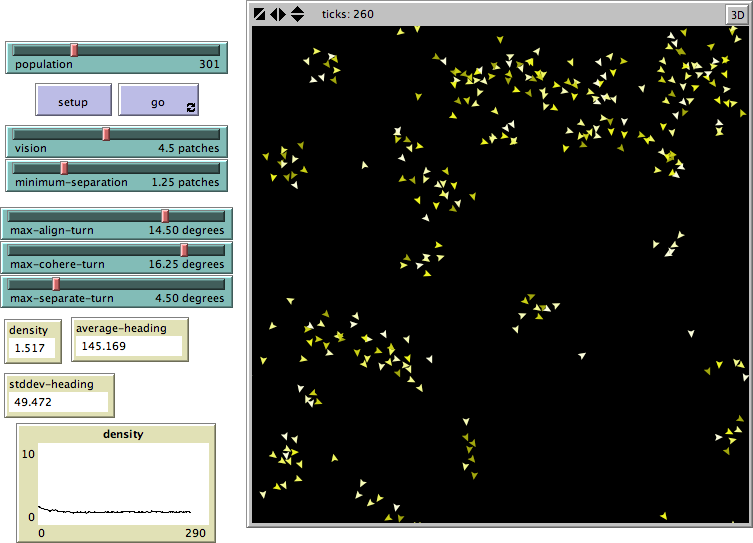
\includegraphics[scale=.5]{images/netlogoui.png}
\caption{A screenshot of NetLogo's graphical user interface while executing a flocking simulation.}
\label{fig:netlogoui}
\end{figure}

% Agent-based control parameters adjust the agent-based programs, but what is interesting is the system-level behavior [diagram]. Example.
% These system-level obvervations are typicall made by the user viewing the visualization of the world.
% Human users can generate a qualitative mapping about a world how the underlying parameters control it.
% Show example [with figures] the difference between two different systems with different qualitative system-level behaviors (boids?)
% Many emergent behaviors can be measured quantitatively to aid the user in understanding the behavior
%  This is done in netlogo with labels... as seen in figure...
Agent-level control parameters adjust the behaviors of agent-based programs.
However, scientists are not typically interested in the local interactions between agents---they are interested in the resulting system-level behaviors that result.
For example, researchers studying agent-based models of lane formations in army ants were interested in the traffic patterns of the lanes, not in the individual behaviors of the ants \cite{couzin2003sol}.
In other work, researchers studying locusts were interested in identifying the critical density at which locusts would begin to swarm and destroy crops \cite{buhl2006dom}.
Typically, scientists analyze ABMs by viewing visualizations of the environment or by gathering statistical data on the simulation.
For instance, NetLogo, an agent-based modeling programming environment \cite{tisue2004netlogo}, provides monitors, plots, and visualizations to convey system-level properties to the user.
In Figure \ref{fig:netlogoui}, monitors are displaying \textit{density}, \textit{average-heading} and \textit{stddev-heading} statistics for a flocking domain.
In addition, a plot of density shows how this property has changed over time.
These tools can be used by researchers to generate a mental model of how the agent-level control parameters of the flocking domain (the sliders seen in the user interface) affect these system-level properties.

% Controlling agent-based models is: unintuitive (learning curve), /elaborate: conceptual disconnect/, example
%   user-time intensive, /elaborate: many sliders/, example
%   difficult to get a high-level view given only the agent-level parameters, /elaborate/, example
Although using ABMs for researching agent-based systems has been proven useful in a number of domains, there is a major conceptual disconnect, from the user's perspective, between the agent-level controls and the system-level properties.
The classical ABM control method of adjusting agent-level properties is unintuitive, because these properties only indirectly affect the system-level properties through emergence.
With the current methodology, a simulation has to be executed in order to observe what the values of the system-level properties will be.
A time-consuming iterative process of guess-and-check is the only way to configure the system to have it exhibit a desired system-level behavior.
Determining what an ABM will do at a system-level, given only the agent-level parameters, is not possible with current software.

% \fw Reduces the learning curve of the system significantly since users are dealing with a control that directly controls the system-level behavior.
% Reduces the amount of time the users physically interacts with the system because they have a reduced number of controls to deal with.
% It is easier to make qualitative determinations from a collection of system-level properties, than the values of the agent-based controls.
%   For example, give a list of agent-level controls and the resultant system-level property values... argue that the system-level property values give more information about the system.
The main goal of the \framework is to bridge the gap between agent-level parameters and system-level properties.
\fw reduces the learning curve of an agent-based model, since users are interacting with the system at the system level, instead of at the agent level.
Qualitative analysis of an ABM's system-level properties will be a more efficient process using \fw, since researchers can interact with an abstraction of the system's controls.
In addition, the models learned by \fw can be inspected to gather quantitative data about the correlations between system-level properties and agent-level parameters.


\section{Wolves, Sheep and Grass}

\begin{figure}[ht]
\centering
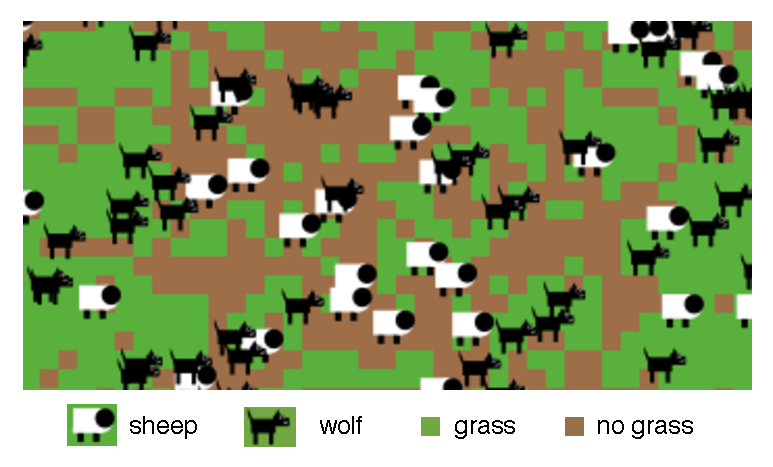
\includegraphics{images/intro_wolfsheep.pdf}
\caption{A screen shot from NetLogo's Wolf Sheep Predation model.}
\label{fig:wolfsheep}
\end{figure}




Throughout this dissertation, I will use NetLogo's Wolf Sheep Predation model \cite{wolfsheep}, which is bundled with NetLogo's standard Model Library,\footnote{http://ccl.northwestern.edu/netlogo/models/WolfSheepPredation} as an example to explain concepts.
A snapshot of its NetLogo visualization is shown in Figure \ref{fig:wolfsheep}.
This multi-agent model simulates a food chain consisting of wolf agents, sheep agents and grass in a two-dimensional space.
The model is controlled by seven agent-level control parameters, which directly affect the following agent behaviors:
\begin{itemize}
  \item The system is initialized with \textit{initial-number-sheep} sheep and \textit{initial-number-wolves} wolves.
  \item Wolves and sheep move randomly though the space.
  \item Wolves and sheep die if they run out of energy.
  \item Wolves eat sheep if they occupy the same space in the environment. Wolves gain \textit{wolf-gain-from-food} units of energy from eating sheep. The sheep dies.
  \item Sheep eat grass if they are on a location of the environment that has grass. Sheep gain \textit{sheep-gain-from-food} units of energy from eating grass. The grass dies in that grid location.
  \item Every time step, each sheep and each wolf has a chance (\textit{sheep-reproduce} and \textit{wolf-reproduce}) to reproduce asexually. Both the parent and the child split the parent's original energy evenly (i.e., the parent's energy divided by two).
  \item Grass regrows after \textit{grass-regrowth-time} number of time steps.
\end{itemize}

\begin{figure}[ht]
\centering
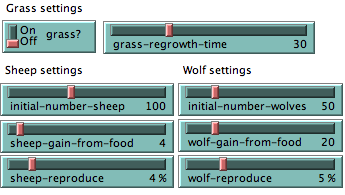
\includegraphics[scale=.66667]{images/wolfsheepcontrols.png}
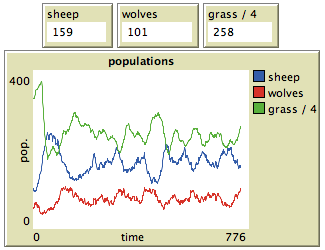
\includegraphics[scale=.66667]{images/wolfsheepmons.png}
\caption{The control and monitor interface for the Wolf Sheep Predation model.}
\label{fig:wolfsheepui}
\end{figure}

The system-level concepts we are interested in are the number of sheep, the number of wolves, and the number of grid locations containing grass.
In NetLogo, these properties are displayed with monitors and a plot, as seen in Figure \ref{fig:wolfsheepui}.
The number of each population of agents may change continuously, but the \textit{average} number of sheep converges.
That is, as more values for the sheep populations are sampled, the average approaches a single value, instead of oscillating like the instantaneous population.
Another interesting feature is that some ecosystems fail: sheep and/or wolves go extinct.

\begin{figure}[ht]
\centering
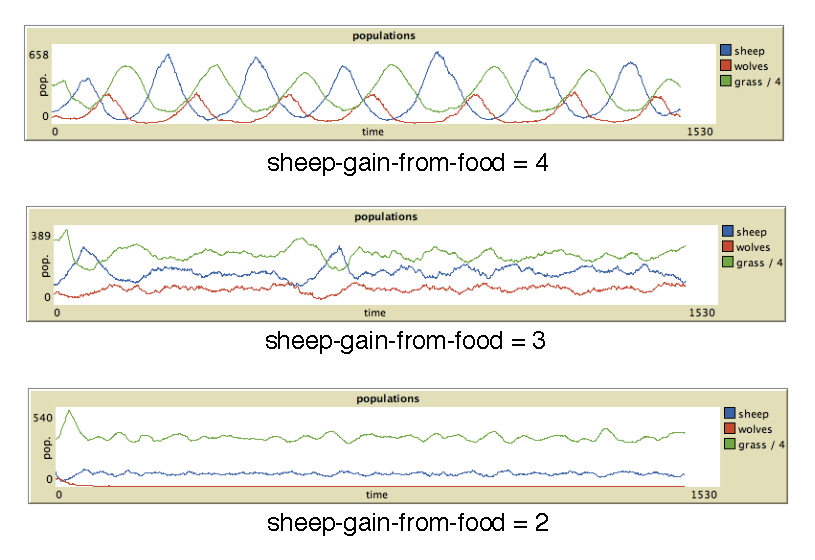
\includegraphics[scale=1]{images/different_sheep.pdf}
\caption{Differences in populations based on changes of the \textit{sheep-gain-from-food} parameter.}
\label{fig:diffsheep}
\end{figure}

After working with this ABM for some time, a user will begin to realize that changes in the control parameters will yield different types of behavior.
For example, by setting \textit{sheep-gain-from-food} to 2, 3, and then 4, major differences in system-level behavior are apparent, as seen in the graphs in Figure \ref{fig:diffsheep}.
When the value of \textit{sheep-gain-from-food} is 4, the system rhythmically exhibits major changes in all three agent populations.
When the value is 2 or 3, the population remains relatively stable, but the average population values are different.
When the value is low enough (e.g., 2) the wolves go extinct.

The Wolf Sheep Predation model is a good example of the intuitive disconnect between agent-level parameters and system-level properties.
There is no clear \textit{explicit} relationship between the controls presented in the user interface and the resulting system-level properties.
An experienced user may have a qualitative understanding of the correlations, but would not be able to predict quantitative concepts, such as the average number of sheep after 2000 time steps (i.e., instantaneous population amounts divided by the number of instantaneous populations sampled).
In  Chapter \ref{Results} (Results), I will show that the intuitive disconnect in this domain can easily be solved by \fw.


\section{Overview of the \framework}


The foundation of this work is framing the problem of building a meta-model of an ABM as two sub-problems: the \textit{forward-mapping problem} and the \textit{reverse-mapping problem}.
In Chapter \ref{ForwardMapping} (The Forward-Mapping Problem), I will discuss how \fw maps given values of the agent-level parameters to expected system-level property values with standard regression approaches.
In Chapter \ref{ReverseMapping} (The Reverse-Mapping Problem), I will discuss how \fw maps a set of desired system-level property values to a set of agent-level parameters that would generate this behavior.
My general approach to solving the reverse-mapping problem is to interpolate configurations using the forward mapping to approximate a smooth and continuous surface.
This interpolated surface represents the space of configurations that would satisfy the system-level requirements set out by the user.
Also, in Chapter \ref{ReverseMapping}, I will discuss alternative methods for solving the reverse-mapping problem.


% The framework consists of four stages: sampling, building the forward mapping, building the reverse mapping, and providing an interface to interact with the models.
% Sampling is done to generate a offline data set to use to train our regression models.
% Next, the relationship between agent-level parameters and quantitative system-level properties are developed.
% This is framed into two problems: the forward mapping problem and the reverse mapping problem.
% Finally, the framework provides standard interfaces and tools to use the two mappings to predict behavior in ABMs and control behavior in ABMs.
\fw is simple and has only a few configuration points.
This allows researchers to focus on the analysis of the system, instead of on the details of \fw.
The framework consists of three major steps: sampling, solving the forward-mapping problem, and solving the reverse-mapping problem.
In these three steps, the only configurations the user must perform are to define how to measure system-level properties of interest, to provide the ranges of parameters to be sampled, and to select a regression algorithm.

I will show in Chapter \ref{Results} that my framework is able to generate models of system-level behavior.
For example, \fw is able to predict the average number of sheep and wolves in the Wolf Sheep Predation model, given the configuration parameter values (the forward-mapping problem).
Also, \fw is able to make suggestions for the values for the control parameters, given the desired system-level property outcome (the reverse-mapping problem).

A more comprehensive overview of \fw is provided in Chapter \ref{Framework}.



\section{Summary of Contributions}

% My contribution is: a \framework that alleviates the common problems in interacting with agent based models, while being domain independent, algorithm independent, and accurate.
%   an indepth look of the problem of building models of agent-based models (meta-models). How do we build them? What properties can they model? How accurately can the behavior of a ABM be predicted and controlled?
%   a learning framework that builds these models and provides users with an interface to the models.
%   I also discuss additional research topics that relate to building and using meta-models.

The main contribution of this dissertation is an in-depth analysis of meta-models of agent-based models.
This analysis includes a discussion of methods for using regression to build models of the correlations between agent-level parameters and system-level properties. 
In addition, this dissertation contains a survey of ways in which meta-models can be used to inspect system-level behaviors of agent-based models.

The \framework encapsulates my methodology for building meta-models of ABMs.
The implementation of \fw serves as a proof-of-concept to show that my approach is feasible and applicable to a variety of domains.
The software itself is a contribution, since it is available to be used by researchers interested in building meta-models of NetLogo ABMs.
The design of the general framework is a contribution as well, since it could be implemented to interact with other agent-based modeling systems similar to NetLogo, or totally independent agent-based models.


\section{Dissertation Organization}

%This dissertation is divided into nine chapters, including this one:
% Chapter Three (Related Work) provides an insight to approaches similar to \fw in motivation.
% Chapter Four (Background) is a survey of concepts in the machine learning literature and agent-based modeling literature that \fw uses.
% Chapters Five and Six define the forward and reverse mapping problems, and give an in depth analysis of how to solve them.
% Chapter Seven (Using Meta-Models) outlines useful ways to use ABM meta-models generated by \fw
% Chapter Eight (Results) surveys a number of experiments I performed to measure the effectiveness of \fw. The experiments are organized by domain, so they also serve as examples of how to apply \fw to ABMs.
% Chapter Nine (Conclusions and Future Work) summarizes this dissertation, provides additional thoughts I have regarding this work and possible directions for future work.
This dissertation is divided into nine chapters, including this one.
Chapter \ref{Framework} The \framework explains each framework component in detail, describes how a new user would tailor \fw to a new ABM, discusses implementation details and gives an introduction to the forward- and reverse-mapping problems.
Chapter \ref{Background} provides information about NetLogo and algorithms used by \fw.
Chapter \ref{Defining} discusses the numerous different ways that system-level properties of ABM can be defined.
Chapter \ref{Domains} enumerates the domains that \fw has been applied to, along with definitions of system-level properties.
Chapters \ref{ForwardMapping} and \ref{ReverseMapping} discuss my solutions to the forward- and reverse-mapping problems.
%Chapter \ref{Using}: Using Meta-Models is a survey of different ways the meta-models generated by \fw can be used to analyze system-level properties of ABMs.
Chapter \ref{Results} evaluates \fw on a domain-by-domain basis and provides explicit examples of how \fw has been used.
Chapter \ref{RelatedWork} compares and contrasts related approaches to \fw.
Chapter \ref{Conclusions} summarizes this dissertation, provides additional discussion and presents possible directions for future work.


 





